\documentclass[12pt]{extarticle}
%\usepackage{times}
\usepackage{geometry}
\usepackage{amsmath,amssymb}
\geometry{a4paper, top=3cm, bottom=3cm, left=2.5cm, right=2.5cm}
%\usepackage[a4paper,top=2.5cm,bottom=2.5cm,left=3cm,right=3cm]{geometry}
\usepackage[utf8]{inputenc}
\usepackage{graphicx}
\usepackage{geometry}
\graphicspath{ {./images/} }
%\usepackage{hyperref}
\usepackage{natbib}
\usepackage{caption}
\usepackage{subcaption}
\usepackage{multirow}
\usepackage[english]{babel}
\usepackage{blindtext}
\usepackage{gensymb}

\providecommand{\abstract}{} 
\providecommand{\abstractname}{Abstract} 
\usepackage{abstract}

\usepackage[english]{babel}

\title{Project details}
\date{}

\begin{document}

\begin{titlepage}

\begin{center}
    \large{\bf ALMA MATER STUDIORUM - UNIVERSITÀ DI BOLOGNA}
    \vspace{2mm}
    \\ \large{\bf \underline{PHYSICS DEPARTMENT}}
    \vspace{5mm}
    \\ \large{Master's degree in:}
    \vspace{5mm}
    \\ \LARGE{Applied Physics}
    \vspace{8mm}
    \\\LARGE{\bf PHYSICAL METHODS OF BIOLOGY}
\end{center}

\vspace{23mm}
\begin{center}
    {\LARGE{CONVOLUTIONAL NEURAL NETWORK \\ FOR WHITE MATTER HYPERINTENSITIES SEGMENTATION \\ \vspace{3mm} 
}}
    
    % Se il titolo è abbastanza corto da stare su una riga, si può usare
    %{\LARGE{\bf Spheroids segmentation\\ \vspace{5mm} per la mia tesi di laurea! }}
    % 
\end{center}
\vspace{50mm}

\begin{minipage}[t]{0.47\textwidth}
	{\large{Supervisors:}{\normalsize\vspace{3mm}
	\bf\\ \large{Prof. Castellani Gastone} \normalsize\vspace{3mm}\bf \\ \large{Dott. Biondi Riccardo}}}
\end{minipage}
\hfill
\begin{minipage}[t]{0.47\textwidth}\raggedleft
	{\large{Candidate:}{\normalsize\vspace{3mm} \bf\\ \large{Ricchi Mattia}}}
\end{minipage}

\vspace{40mm}
\hrulefill
\\\centering{\large{YEAR 2022}}

\end{titlepage}

\renewcommand{\abstractname}{Abstract}

\newpage
\section{Introduction}
White matter hyperintensities (WMH) are signal abnormalities of white matter on T2-weighted magnetic resonance imaging (MRI) sequence.
As MRI has become widely available and brain magnetic resonance imaging is increasingly being carried out in various clinical settings, clinicians often have to deal with the incidental discovery of white matter lesions, appearing as hyperintensities on T2-weighted images, in particular in FLAIR sequence MRI.
These lesions are located in the deep white matter and are often seen together with vessels affected by small vessel disease \cite{ventricular_lesions}.
Several studies have assessed the relationship between white matter hyperintensities and the insurgence of several pathologies, leading to the conclusion that white matter hyperintensities predict an increased risk of stroke, dementia, and death \cite{wmh}. Therefore, when identified as part of diagnostic investigations, they indicate an increased risk of cerebrovascular events. 
For these reasons, early identification of white matter lesions is of extremely high importance.\\[4pt]
Manual segmentation is currently the gold standard to evaluate the volume of WMH, but it is time-consuming and subject to intra and inter-operator variability \cite{manual}.
Therefore, this work aims to provide an algorithm to automatically detect and segment such white matter hyperintensities using fluid-attenuated inversion recovery (FLAIR) and T1 magnetic resonance scans.
The method used in this work is based on a deep fully convolutional neural network and ensemble model, thus a machine learning technique for the automatic diagnosis of diseases through medical imaging. 

\begin{figure}[h!]
    \centering
    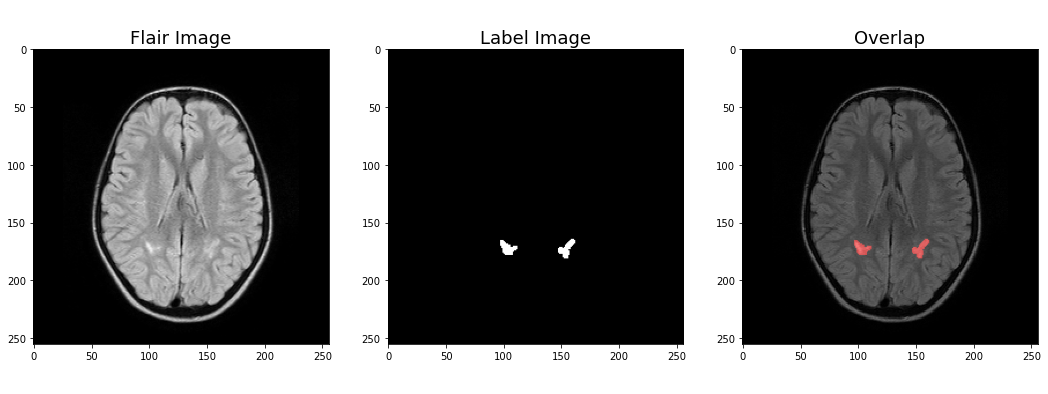
\includegraphics[width = \textwidth]{images/overlap.png}
    \caption{Example of manual segmentation of WMH}
    \label{fig:manual_seg}
\end{figure}
\noindent
U-Net architecture is designed for semantic segmentation, which means that in the final image, each pixel either represents the detected object or the background.
The architecture, an example of which is shown in Figure \ref{fig:unet}, consists of a contracting path to capture
context and a symmetric expanding path that enables precise localization \cite{unet}.
The two paths are concatenated with each other and this concatenation of feature maps is what gives localized information, thus making semantic segmentation possible.
The contracting path follows the typical architecture of a convolutional network \cite{unet}. It consists of the repeated application of convolutions, which is nothing but a matrix multiplication, each followed by a rectified linear unit (ReLU) and a max pooling operation, which consists in scanning a small matrix over the image, within that matrix the maximum value is selected and replaced inside the small matrix itself.
Every step in the expansive path consists of an upsampling of the feature map followed by a convolution, called “up-convolution”, that halves the number of feature channels, a concatenation with the correspondingly cropped feature map from the contracting path, and other convolutions, each followed by a ReLU \cite{unet}. The cropping is necessary due to the loss of border pixels in every convolution.
Of course, the parameters of the network may change depending on the task it has to perform but the overall structure remains invariant.
In general, convolutional neural networks have proven to be an effective computational model for automatically extracting image features. \\[4pt]
The aim of this work concerns the detection and segmentation of WMH in MR images of patients affected by sickle cell disease.
The used approach is based on an ensemble of convolution-deconvolution architecture which simultaneously classifies each pixel and locates objects of an input image \cite{fully_conv}.
The training of the networks of the ensemble model is performed using the hardware offered by CINECA, in particular using the MARCONI-100 supercomputer.

\section{Materials and Methods}
\subsection{Dataset}
The dataset consists of $61$ magnetic resonance brain volumes of patients affected by sickle cell disease. The images were acquired with both FLAIR and T1W modalities. Each volume is divided into several axial slices, for a total of $5562$ slices. As shown in Figure \ref{fig:dataset_example}, aside from the FLAIR and T1W slices, each slice is provided together with the segmentation of the brain area, which constitutes the binary brain mask, and with the label mask, a binary image that contains the manual segmentation of the white matter hyperintensities. \\
All the images are registered in a common space, but the gray level intensities are not normalized. For this reason, further preprocessing of the images is required.\\
Among the volumes provided, $55$ are used as training samples while the remaining $6$ are used for testing. 
\begin{figure}[h!]
    \centering
    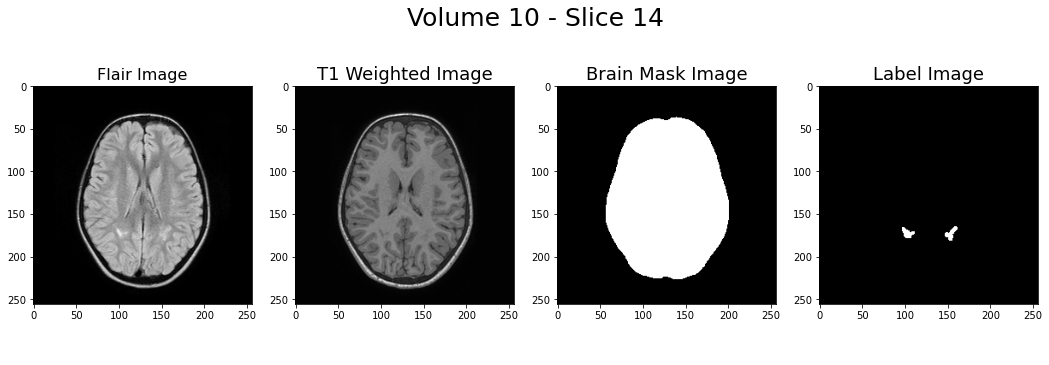
\includegraphics[width = \textwidth]{images/dataset_example.png}
    \caption{Example of an axial slice of the dataset.}
    \label{fig:dataset_example}
\end{figure}

\subsection{Image preprocessing}
Since the slice dimensions vary from subject to subject and since the image intensity is not normalized, further preprocessing on top of the basic preprocessing steps performed by the image provider is required for several reasons.
Firstly, to guarantee a uniform size of all the slices for deep convolutional networks in the training and testing step. Moreover, the normalization of the voxel intensity is needed to reduce variation across subjects. \\
To perform the just mentioned steps, an algorithm has been implemented in Python that automatically crops all the slices to $256\times256$ to guarantee a uniform size for input to the model. In addition to that, the algorithm also performs a Gaussian normalization to rescale the voxel intensities within each individual's brain mask. \\
Finally, since the U-Net takes as input an image with two channels, that are respectively the FLAIR and the T1W images, for each slice of each patient the correspondent FLAIR and T1W images are concatenated together, obtaining a final image with dimensions $(256, 256, 2)$. In this way, the FLAIR and T1 modalities are fed into the U-Net jointly as a two-channel input for each patient.

\subsection{Data augmentation}\label{sec:data_aug}
Data augmentation is a technique that can be used to artificially expand the size of a training set by creating modified data from the already existing one. 
In fact, in machine learning, the situation when the model does not generalize well from the training data to unseen data is called overfitting, which is one of the trickiest obstacles in applied machine learning.
One solution to overcome this problem is to train the network with more data. 
Data augmentation is typically used to prevent overfitting, but also when the dataset is too small to train on. \\
The typical techniques used in data augmentation are Geometric transformations, to randomly flip, crop, rotate or translate images, Kernel filters, to sharpen or blur an image, and also Random Erasing, to delete a part of the initial image, and Mixing images, to mix images with one another. \\[4pt]
In this work, simple transformations are used in order to augment data, such as a random rotation of an angle uniformly distributed between $-15\degree$ and $15\degree$, a random scaling of the image in the vertical and horizontal directions with coefficients uniformly distributed in the interval $[0.9, 1.1]$, and a random shearing of the image with coefficient uniformly distributed between $-0.1$ and $0.1$. An example of data augmentation result is shown in Figure \ref{fig:data_aug}.\\
The choice of the applied transformations is based on the fact that in the case of MR images among different subjects and scanners, due to variations of head orientation, voxel sizes and WMH distribution, the algorithm needs to acquire robustness to subject rotation and to shear transformations. \\[4pt]
Since the training images containing lesions are just a small part of the overall training set, the data augmentation is applied only to those images containing WMH, and from each slice, ten new slices are obtained, thus sensibly increasing the size of the training dataset.
\begin{figure}[h!]
    \centering
    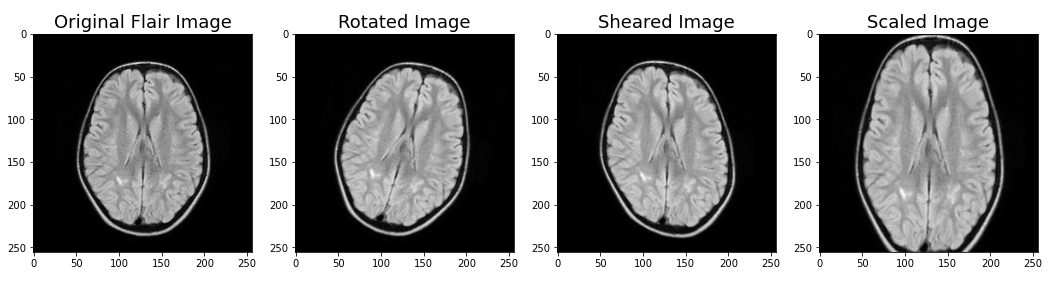
\includegraphics[width = \textwidth]{images/data_augmentation.png}
    \caption{Example of data augmentation result. From left to right: the original axial slice, slice after rotation, slice after shear mapping and slice after scaling.}
    \label{fig:data_aug}
\end{figure}

\subsection{U-Net architecture and Ensemble Model}\label{sec:unet arch}
The U-Net used in this work is based on the one implemented in the article \textit{Fully convolutional network ensembles for white matter hyperintensities segmentation in MR images} \cite{fully_conv}. The network, shown in Figure \ref{fig:unet}, consists of a down-convolutional part that shrinks the spatial dimensions (left side) and an up-convolutional part that expands the score maps (right side).
Two convolutional layers are repeatedly employed, each followed by a rectified linear unit (ReLU) and a $2\times 2$ max pooling operation with stride $2$ for downsampling \cite{fully_conv}. At the final layer, a $1\times 1$ convolution is used to map each $64-$component feature vector to two classes \cite{fully_conv}. In total the network contains $19$ convolutional layers. 

\begin{figure}[h!]
    \centering
    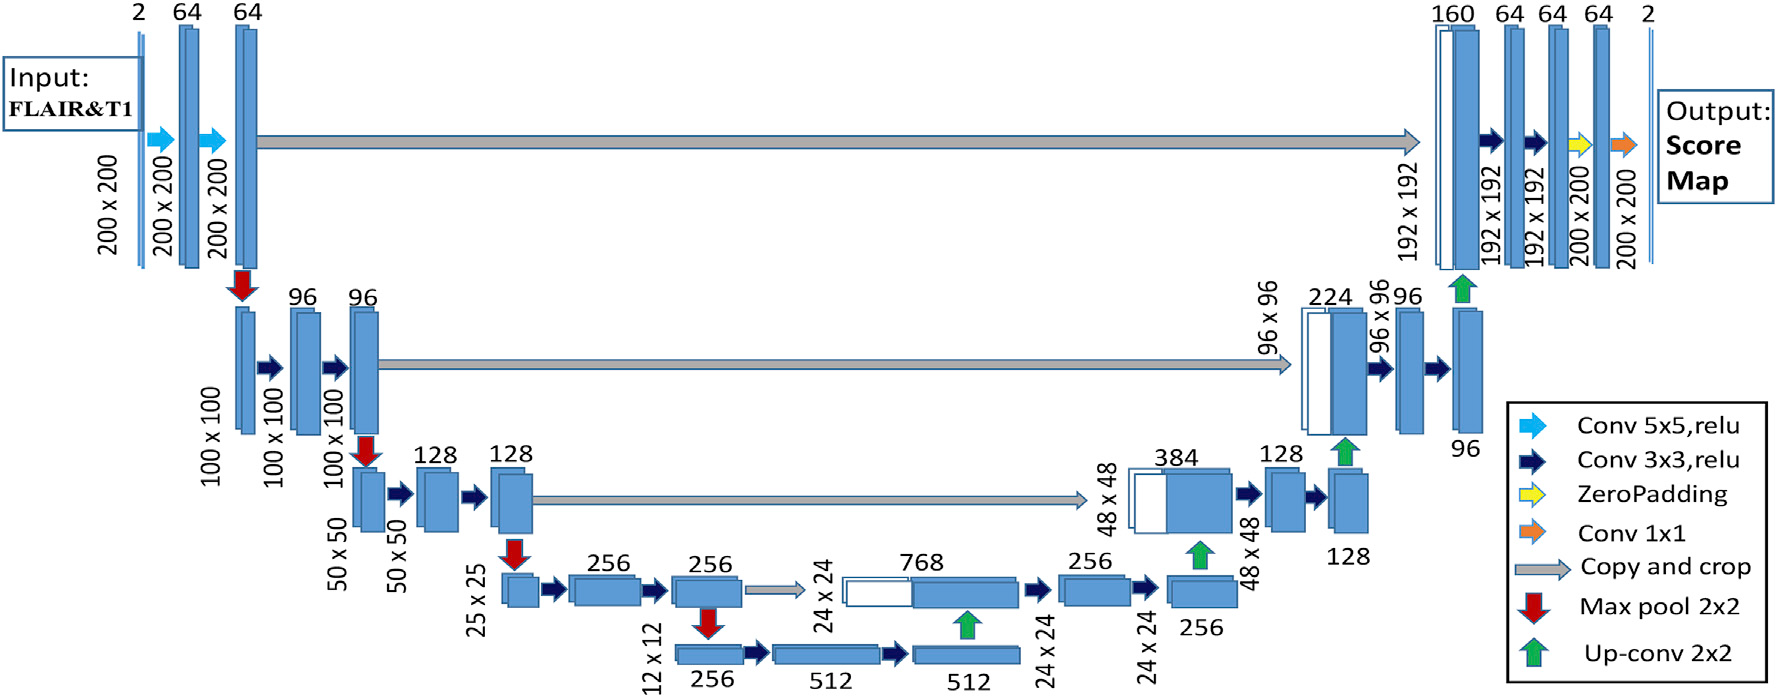
\includegraphics[width = \textwidth]{images/U-Net.png}
    \caption{2D Convolutional Network Architecture. It consists of a shrinking part (left side) and an expansive part (right side) to detect and locate WMH respectively. The input includes FLAIR and T1 channels. Image courtesy by \cite{fully_conv}.}
    \label{fig:unet}
\end{figure}
\noindent
Ensemble techniques combine multiple learning models to obtain better predictive results than the single constituents learning algorithm alone. By using these techniques, the overfitting problems of complex models are reduced since different models could learn different aspects of the training data during the learning process \cite{fully_conv}. 
In this work, three different U-Net models with the same architecture are trained and, when given a test image, for each of the three models, a segmentation map is generated as a result. As a final step, the resulting three maps are averaged and, finally, an empirical threshold is used to transform the probability map into a binary segmentation map.

\subsection{Loss functions and parameters}\label{sec:loss_and_param}
Loss functions are mathematical equations that calculate how far the predictions deviate from the actual values. 
Higher loss values suggest that the model is making a significant error, whereas lower loss values imply that the predictions are rather accurate. 
The goal is to reduce the loss function as much as possible. 
The loss function is used by models to learn the trainable parameters, such as weights and biases.\\[4pt]
In the task of WMH segmentation, the numbers of positives and negatives are highly unbalanced. One possible solution to tackle this issue is to use the Dice Loss as the loss function for training the model. As defined in \cite{fully_conv}, the formulation for the Dice Loss is as follows.
Let $G=\{g_1, \dots, g_N\}$ be the ground-truth segmentation probabilistic maps over $N$ slices, and $P=\{p_1, \dots ,p_N\}$ be the predicted probabilistic maps over $N$ slices. The Dice Loss function can be expressed as:
\begin{equation}
	DL = -\dfrac{2 \sum_{n=1}^N \left| p_n \circ g_n \right| + s}{\sum_{n=1}^N \left( \left| p_n \right| + \left| g_n \right| \right) + s}
\end{equation}
where $\circ$ represents the entrywise product of two matrices, and $\left| \cdot \right|$ represents the sum of the entries of matrix.
The $s$ term is here used to ensure the loss function stability by avoiding the division by $0$; in this work it is set to $1$.\\[4pt]
Another loss function used in this work is the Binary Focal Loss. 
This loss function, defined in Equation \eqref{eq:focal_loss} generalizes binary cross-entropy by introducing a hyperparameter $\gamma$, called the focusing parameter, that allows hard-to-classify examples to be penalized more heavily relative to easy-to-classify examples.
In other words, focal loss focuses on the examples that the model gets wrong rather than the ones that it can confidently predict, ensuring that predictions on hard examples improve over time rather than becoming overly confident with easy ones. The Binary Focal Loss can be defined as:
\begin{equation}
    L(y, \hat{p})= - \alpha y (1-\hat{p})^{\gamma} - (1-y)\hat{p}^{\gamma}log(1-\hat{p})
    \label{eq:focal_loss}
\end{equation}
\noindent
In Equation \eqref{eq:focal_loss}, $y \in [0, 1]$ is the binary class label, $\hat{p} \in [0, 1]$ is an estimate of the probability of the positive class, $\gamma$ is the focusing parameter, the higher the $\gamma$, the higher the rate at which easy-to-classify examples are down-weighted, and $\alpha$ is a hyperparameter that governs the trade-off between precision and recall by weighting errors for the positive class up or down. \\[4pt]
Another loss function that is used in this work is the Focal Tversky Loss, a generalization of the Tversky Index (TI). The TI is an asymmetric similarity measure that is a generalisation of the dice coefficient, and is defined as follows:
\begin{equation}
 TI = \dfrac{TP}{TP+\alpha \cdot FN + (1-\alpha)\cdot FP}
 \label{eq:tversky_index}
\end{equation}

\noindent where $TP$ is the number of true positives, $FN$ the number of false negatives and $FP$ the number of false positives in the final segmented image. The TI also introduces a parameter $\alpha$ which is used to penalise more false positives or false negatives: by setting $\alpha > 0.5$, the model will penalise false negatives more. 
This becomes useful in highly imbalanced datasets where the additional level of control over the loss function yields better small scale segmentations than the normal dice coefficient.\\[4pt]
The Focal Tversky Loss (FTL) is a generalisation of the tversky loss. The non-linear nature of the loss gives you control over how the loss behaves at different values of the tversky index obtained.
\begin{equation}
FTL = \left( 1 - TI \right) ^{\gamma}
\label{eq:focal_tversky}
\end{equation}
In Equation \eqref{eq:focal_tversky}, the $\gamma$ parameter is used to control the non-linearity of the loss: with a value of $\gamma < 1$, the gradient of the loss is higher for examples where $TI > 0.5$, forcing the model to focus on such examples.
In the case of class imbalance, the FTL becomes useful when $\gamma > 1$. This results in a higher loss gradient for examples where $TI < 0.5$. This forces the model to focus on harder examples, especially small scale segmentations which usually receive low TI scores.\\[6pt]
When building a new machine learning algorithm, one has to face with the choice of a series of parameters that will determine and influence the working and performance of the algorithm itself. 
One of the most important parameters is the Learning Rate, a tuning parameter in the optimization algorithm that determines the step size at each iteration while moving toward a minimum of a loss function.
In other words, it metaphorically represents the speed at which a machine learning model learns.
Remembering that the aim is to find the minimum of the loss function, a too high learning rate will make the learning jump over minima but a too low learning rate will either take too long to converge or get stuck in an undesirable local minimum \cite{deep_learning}.\\
In order to achieve faster convergence, prevent oscillations and getting stuck in undesirable local minima the learning rate is often varied during training either in accordance to a learning rate schedule or by using an adaptive learning rate. In this work, a learning rate schedule is used to change the learning rate during training between two consecutive epochs. 
There are many different learning rate schedules but the one used to train the network is the exponential one, which exponentially decreases the learning rate as the number of epochs increases. 
The mathematical formula which describes this learning rate schedule is:
\begin{equation}
\eta_n = \eta_{n-1} \cdot e^{-d}
\label{eq:LRscheduler}
\end{equation}
In Equation \eqref{eq:LRscheduler}, $\eta$ represents the learning rate, $n$ the epoch number and $d$ is a decay parameter. \\[4pt]
Another parameter that needs to be set for fitting and training the model is the Validation Split. This parameter accepts any number between $0$ and $1$ and it represents the fraction of the training data to be used as validation data. 
The model will set apart this fraction of the training data, will not train on it, and will evaluate the loss and any model metrics on this data at the end of each epoch. \\[4pt]
In implementing a machine learning algorithm, one could also use the Early Stopping, a form of regularization used to avoid overfitting when training the network with an iterative method, such as the gradient descent method.
This method is related to the fact that too little training of the network will mean that the model will underfit the train and the test sets. Too much training will mean that the model will overfit the training dataset and have poor performance on the test set.
A compromise is to train on the training dataset but to stop training at the point when performance on a validation dataset starts to degrade.
Early stopping rules provide guidance as to how many iterations can be run before the learner begins to over-fit.

\subsection{Evaluation metric}\label{sec:evaluation_metric}
The \emph{Dice similarity coefficient}, also known as the Sørensen–Dice index or simply Dice coefficient, is a statistical tool which measures the similarity between two sets of data and has become arguably the most broadly used tool in the validation of image segmentation algorithms.\\
Given a ground-truth segmentation map $G$ and a segmentation map P generated by the algorithm, the Dice similarity coefficient $DSC$ is defined as:
\begin{equation}
DSC = \dfrac{2\left( G \cap P  \right)}{\left| G \right| + \left| P \right|}
\end{equation}
This evaluation metric measures the spatial overlap in percentage between $G$ and $P$.
As explained in \cite{dice_coef}, the $DSC$ value is a simple and useful summary measure of spatial overlap, which can be applied to studies of reproducibility and accuracy in image segmentation.\\
The $DSC$ can assume values in the interval $\left[ 0 , 1 \right]$: $DSC=0$ means no overlap, $0<DSC<1$ implies partial overlap while $DSC=1$ indicates complete overlap between the two segmentation maps.\\[4pt]
Lesion Recall is another metric that will be used in this work to evaluate the performance of the segmentation algorithm. This metric represents the fraction of pixels that is correctly identified by the model and is based on the number of true positives $TP$ and false negatives $FN$. More precisely, it is the number of true positive results divided by the number of all samples that should have been identified as positive:
\begin{equation}
Recall = \dfrac{TP}{TP+FN}
\label{eq:recall}
\end{equation}

\noindent As it can be understood from Equation \eqref{eq:recall}, a model that does not produce false negatives has a Recall equal to $1.0$.\\[4pt]
A similar metric that can be defined is the Precision, that is the number of true positive results divided by the number of all positive results, including those not identified correctly: 
\begin{equation}
Precision = \dfrac{TP}{TP+FP}
\label{eq:precision}
\end{equation}

\noindent Finally, F1 score, defined in Equation \eqref{eq:f1}, is the harmonic mean of the precision and recall. It thus symmetrically represents both precision and recall in one metric. The highest possible value of an F-score is 1.0, indicating perfect precision and recall, and the lowest possible value is 0, if either precision or recall are zero.
\begin{equation}
F1 =2 \dfrac{Precision \cdot Recall}{Precision+Recall}=\dfrac{2TP}{2TP+FP+FN}
\label{eq:f1}
\end{equation}

\section{Results and Discussion}\label{sec:results}
To begin with, the first results that are presented in this section are the segmentation results obtained without training the network. 
In Figure \ref{fig:DSC_beforeTraining} is shown the $DSC$ for the six different test volumes.
\begin{figure}[h!]
\centering
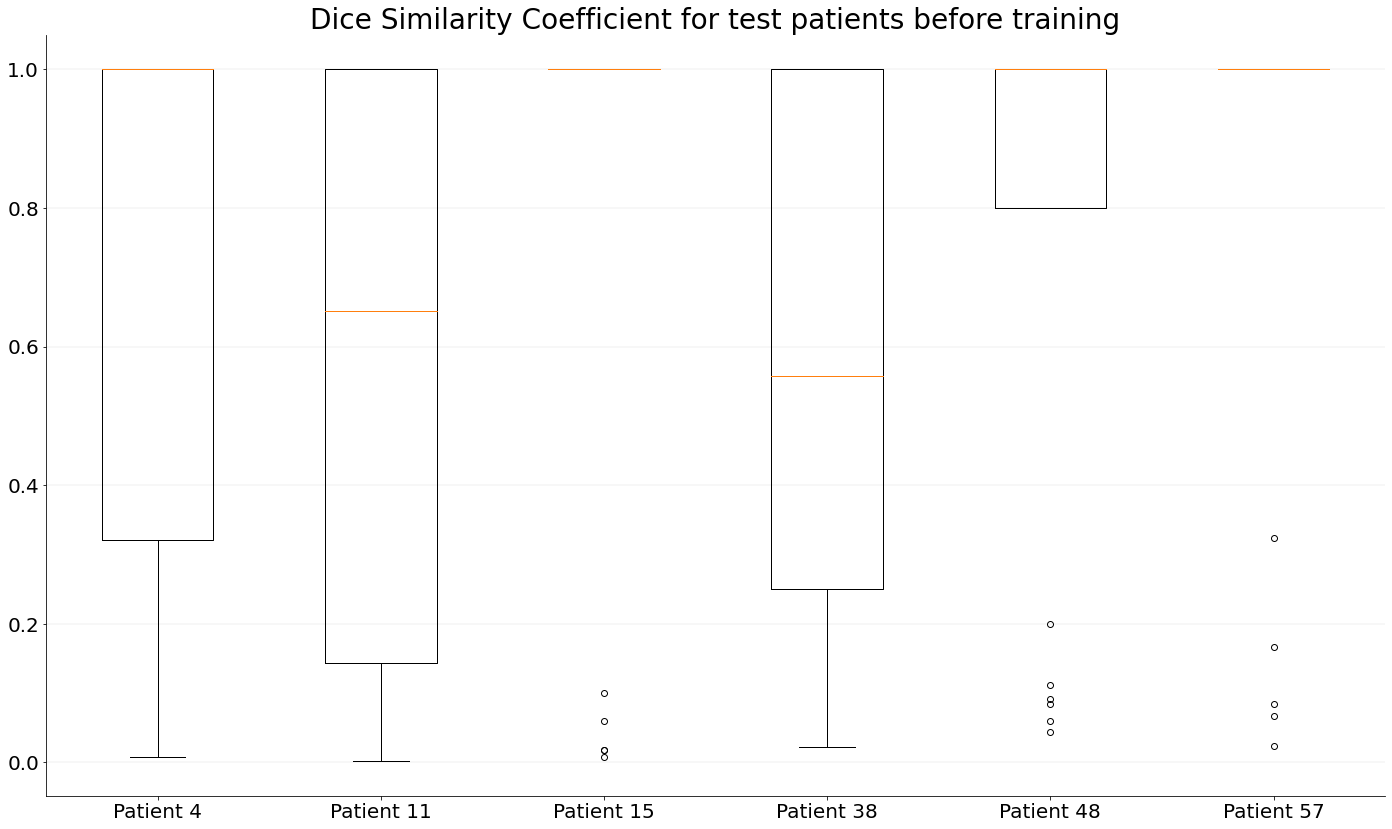
\includegraphics[width = \textwidth]{DSC_beforeTraining.png}
\caption{Dice Similarity Coefficient for the test volumes before training the network.}
\label{fig:DSC_beforeTraining}
\end{figure}

\noindent As one can observe from Figure \ref{fig:DSC_beforeTraining}, the $DSC$ also covers very low values, smaller than $0.2$, remarking the very poor results that the model provides before being trained.
\begin{figure}[h!]
\centering
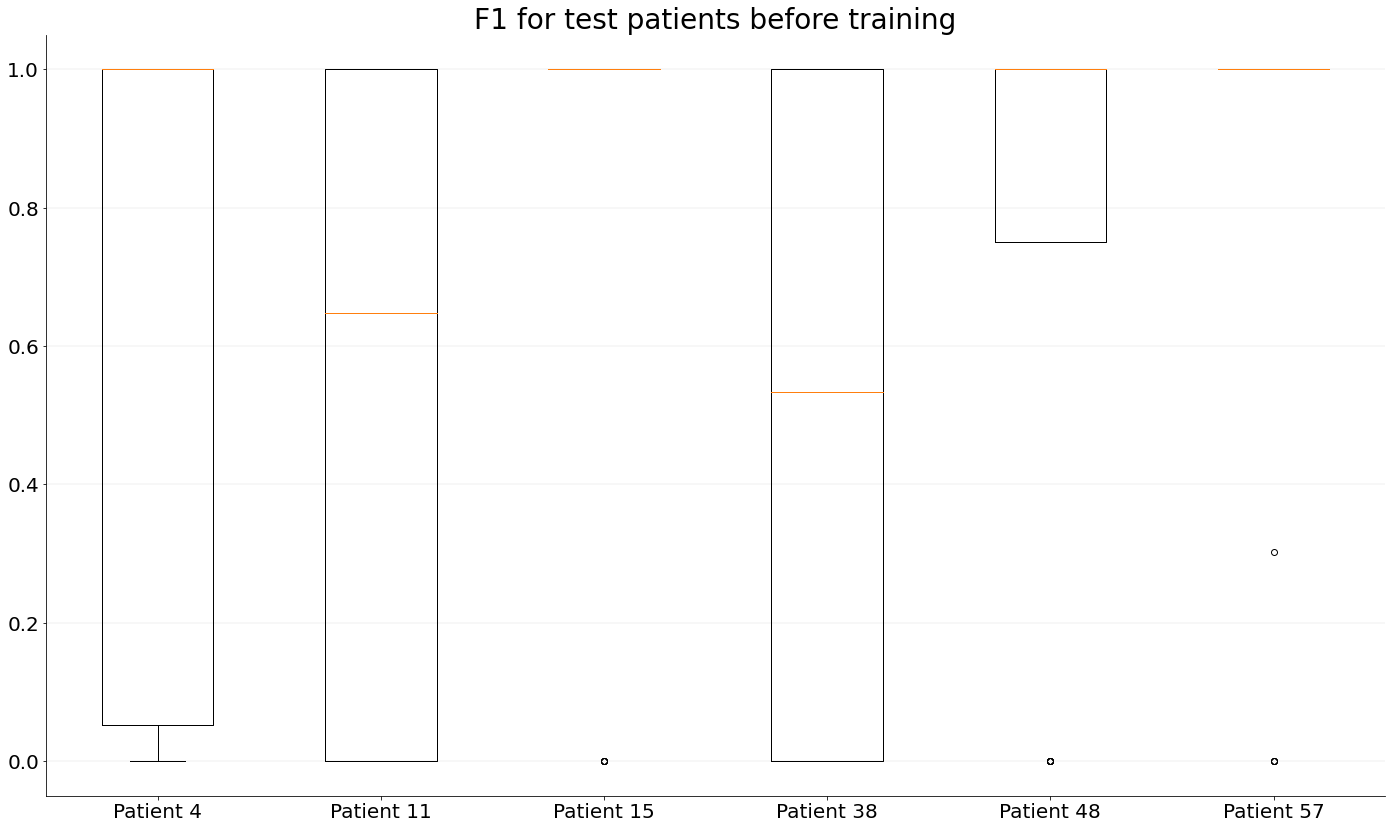
\includegraphics[width = \textwidth]{F1_beforeTraining.png}
\caption{F1 score for the test volumes before training the network.}
\label{fig:F1_beforeTraining}
\end{figure}

\noindent In Figure \ref{fig:F1_beforeTraining} is shown the box-plot of the F1 score before training the network for all the test volumes, showing very low values which represent a high rate of false positives and/or false negatives.\\[4pt]
As mentioned in Section \ref{sec:unet arch}, in this work an ensamble model has been used. In particular, three models have been implemented and concatenated with each other, each of which constitutes of a U-Net architecture: the first model uses the Dice Loss function as a loss function with a learning rate of $10^{-5}$; in the second model it is the Focal Tversky Loss that plays the role of the loss function, with $\alpha = 0.7$, $\beta = 0.3$ and $\gamma = 4$, with a learning rate of $10^{-6}$; finally, the third model has the Binary Focal Loss as a loss function with the focusing parameter $\gamma$ equals to $2$ and a learning rate of $10^{-6}$.\\
For all the three models, a learning rate scheduler has been used in order to reduce the learning rate within the training session, as the number of the epoch increases. The learning rate scheduler used in this work is the exponential one, explained by Equation \eqref{eq:LRscheduler} and with a decay parameter $d$ equal to $0.1$.
\begin{figure}[h!]
\centering
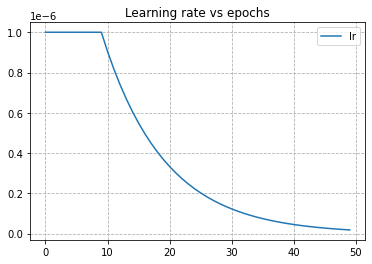
\includegraphics[scale = 0.8]{LR.png}
\caption{Learning Rate as a function of the epoch number.}
\label{fig:LR}
\end{figure}
As it can be seen from Figure \ref{fig:LR}, the learning rate remains constant for the first $10$ epochs and then it decreases exponentially, potentially preventing the overfitting of the model.\\[4pt]
Another callback used in this work is the Early Stopping, with the aim of preventing the overfitting of the model. The function that is monitored is set to be the validation loss with a patience of $5$ epochs. This means that the validation loss is continuously evaluated and, if after $5$ epochs the performance of the model does not improve, the training is stopped.\\[4pt]
Moreover, in order to improve the performance of the model, only the slices containing white matter lesions are considered in the training dataset. The final results of the network are evaluated with the Dice similarity coefficient, Precision, Recall and F1 score, all explained in Section \ref{sec:evaluation_metric}. 

\begin{figure}[h!]
     \centering
     \begin{subfigure}[b]{0.45\textwidth}
         \centering
         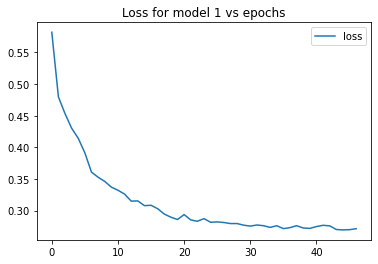
\includegraphics[width=\textwidth]{loss_model1.png}
         \caption{Model 1}
         \label{fig:loss_model1}
     \end{subfigure}
     \hfill
     \begin{subfigure}[b]{0.45\textwidth}
         \centering
         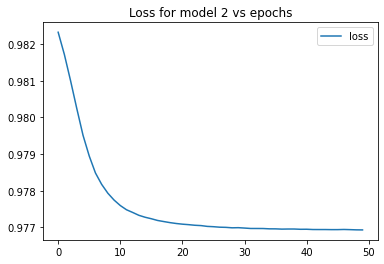
\includegraphics[width=\textwidth]{loss_model2.png}
         \caption{Model 2}
         \label{fig:loss_model2}
     \end{subfigure}
     \hfill
     \begin{subfigure}[b]{0.45\textwidth}
         \centering
         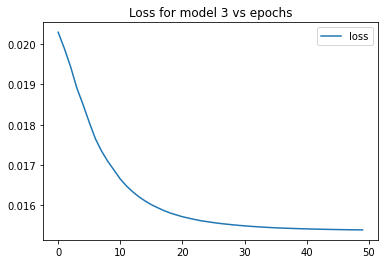
\includegraphics[width=\textwidth]{loss_model3.png}
         \caption{Model 3}
         \label{fig:loss_model3}
     \end{subfigure}
        \caption{Loss function for the three models as a function of the epoch number.}
        \label{fig:loss_models}
\end{figure}

\noindent In Figure \ref{fig:loss_models} are shown the three loss functions vs the epoch number. As expected, the loss function decreases as the epoch number increases. Also for model 1, in Figure \ref{fig:loss_model1}, the Early stopping ended the training session before the 50th epoch as the loss function did not improve in the previous five epocs.

\begin{figure}[h!]
\centering
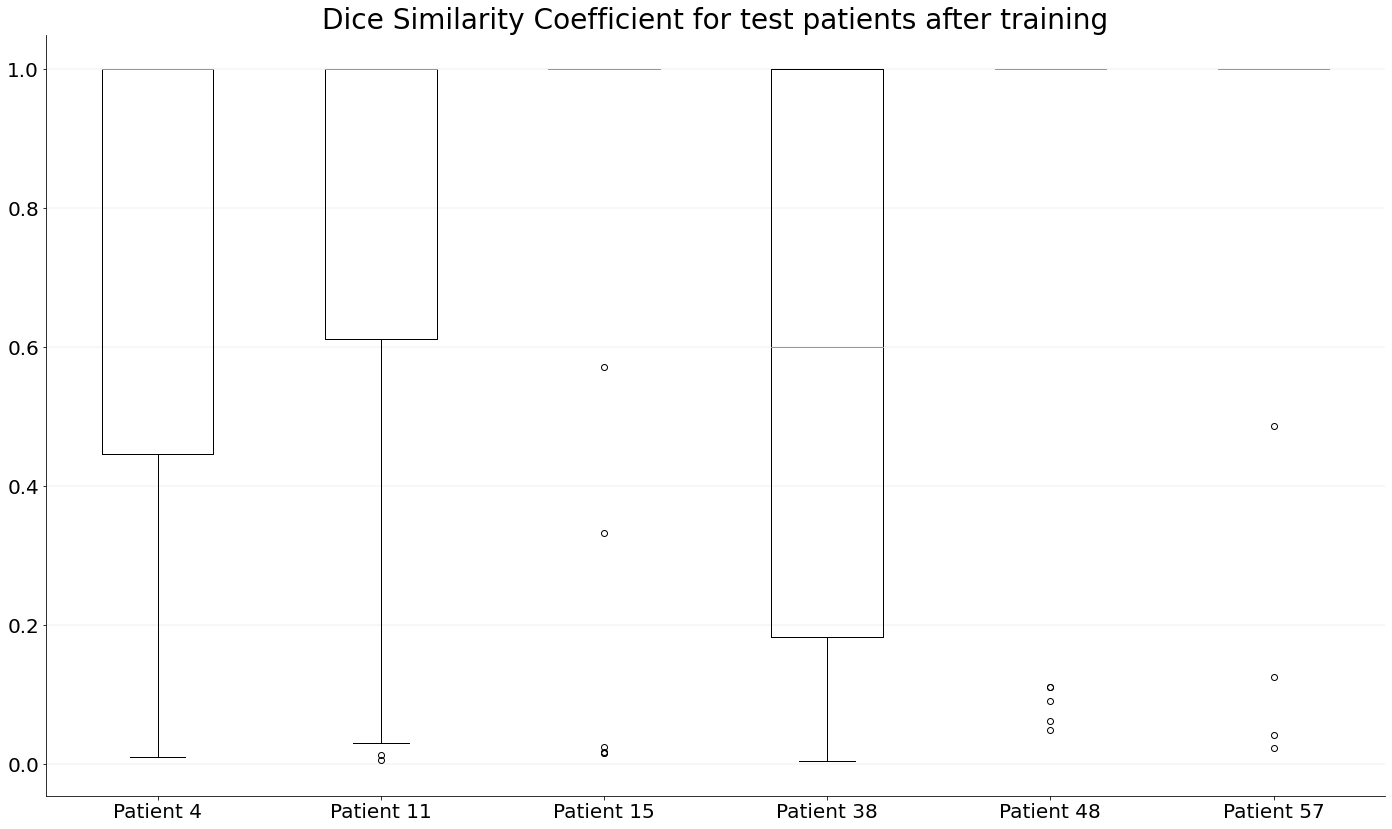
\includegraphics[width = \textwidth]{DSC_afterTraining.png}
\caption{Dice Similarity Coefficient for the test volumes after training the network.}
\label{fig:DSC_afterTraining}
\end{figure}
\vspace{6pt}
\noindent In Figure \ref{fig:DSC_afterTraining} is shown the Dice Similarity Coefficient after the training session of the model. As it can be noticed by comparing Figure \ref{fig:DSC_beforeTraining} and Figure \ref{fig:DSC_afterTraining}, the model provides with better results since the distribution of the DSC has reduced to values closer to $1$, and also the number of outliers has decreased. Only for patient 38, it can be observed that the performance of the model actually got sightly  worse after training. \\
However, some bad results are still present with a DSC very close to zero. 

\begin{figure}[h!]
\centering
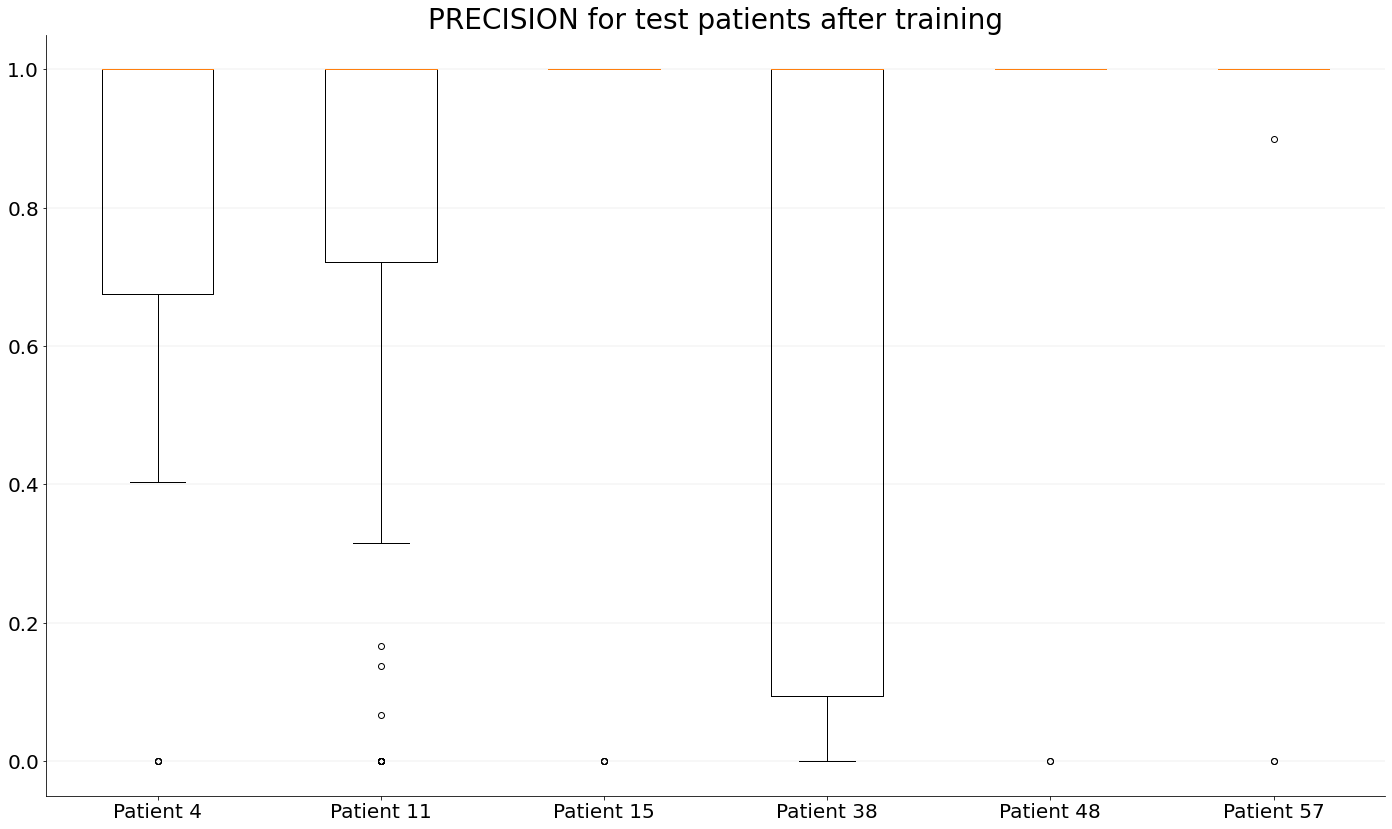
\includegraphics[width = \textwidth]{PRECISION_afterTraining.png}
\caption{Precision for the test volumes after training the network.}
\label{fig:PRECISION_afterTraining}
\end{figure}

\begin{figure}[h!]
\centering
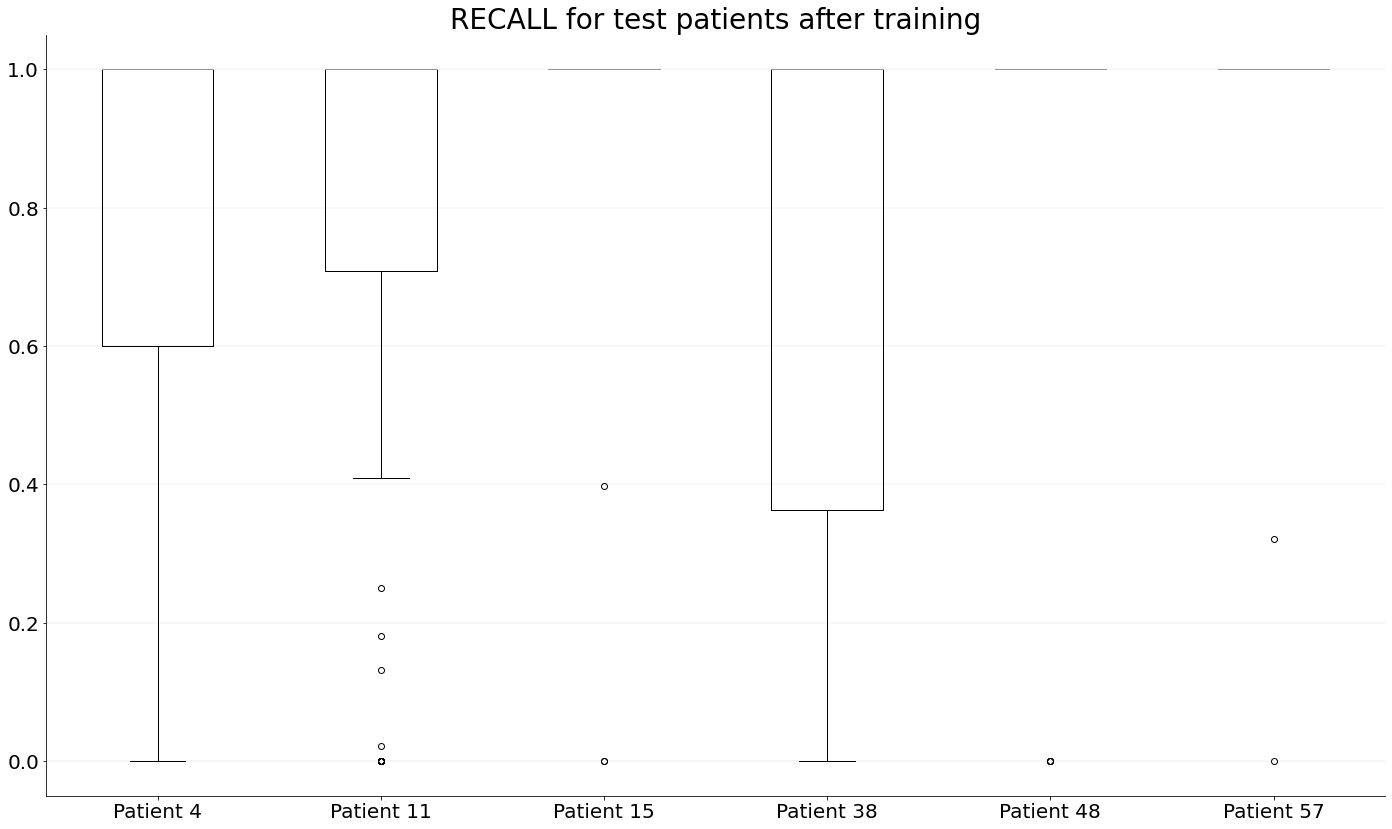
\includegraphics[width = \textwidth]{RECALL_afterTraining.png}
\caption{Recall for the test volumes after training the network.}
\label{fig:RECALL_afterTraining}
\end{figure}

\begin{figure}[h!]
\centering
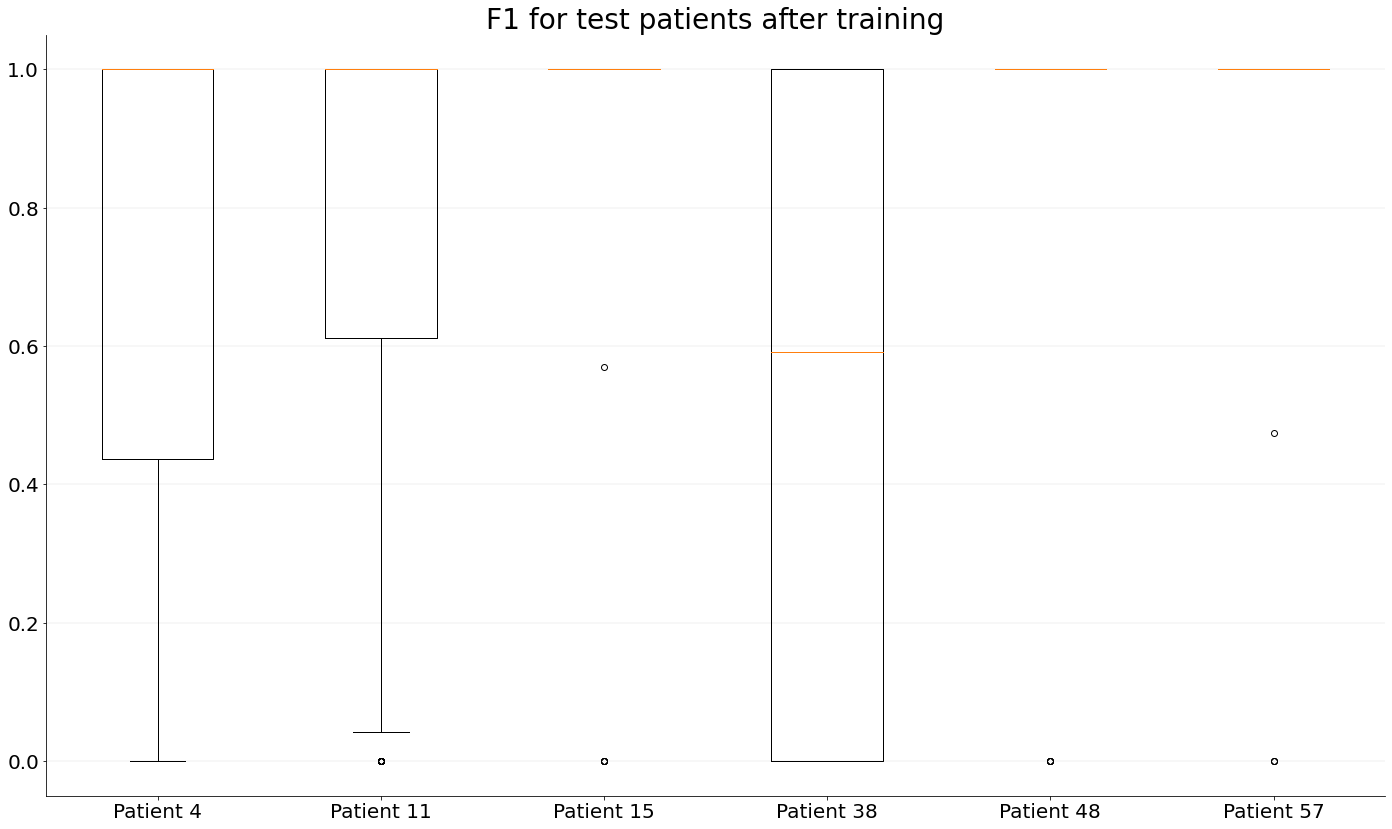
\includegraphics[width = \textwidth]{F1_afterTraining.png}
\caption{F1 score for the test volumes after training the network.}
\label{fig:F1_afterTraining}
\end{figure}

\noindent In Figure \ref{fig:PRECISION_afterTraining}, Figure \ref{fig:RECALL_afterTraining} and Figure \ref{fig:F1_afterTraining} are shown respectively the precision, the recall and F1 score of the model after being trained.
Similar considerations can be done as for the DSC: quite good results have been obtained with a few outliers. However, for patient 38, no improvement of the performance of the model has been obtained.

\begin{figure}[h!]
\centering
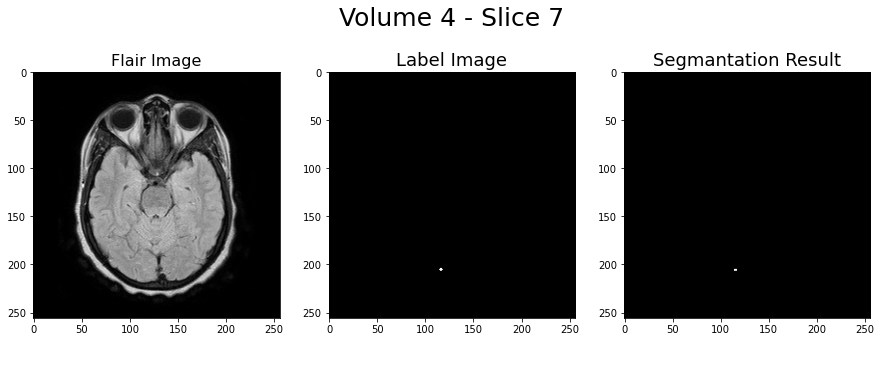
\includegraphics[width = \textwidth]{volume-004-007.png}
\caption{Segmentation result for slice 7 of patient 4.}
\label{fig:volume-004-007}
\end{figure}
\vspace{6pt}
\noindent In Figure \ref{fig:volume-004-007} it is shown a segmentation result for slice 13 of patient 4. It can be seen how a particularly small lesion has been correctly identified and segmented in the final image.\\[4pt]
Another good result for patient 4 has been obtained in slice 14, shown in Figure \ref{fig:volume-004-014}. In this case, two WMH have been correctly identified and segmented, but one of the two in the final result appears smaller than the actual lesion, contributing to decrease the DSC and F1 score.\\[4pt]
In Figures \ref{fig:volume-011-150} and \ref{fig:volume-011-140} are shown two other results for patient 11 in which the model performed well, identifying and segmenting correctly the white matter lesions. Nevertheless, a few false positives and false negatives are present.\\[4pt]
Concerning patient 38, some quite good results have been obtained, an example of which is shown in Figure \ref{fig:volume-038-151}. However, the fast majority of the slices do not show a good segmentation result, like in Figure \ref{fig:volume-038-147}. In this case in particular, the WMH has been correctly segmented but it has also been identified as a lesion another large area of white matter which instead is not a WMH.


\begin{figure}[h!]
\centering
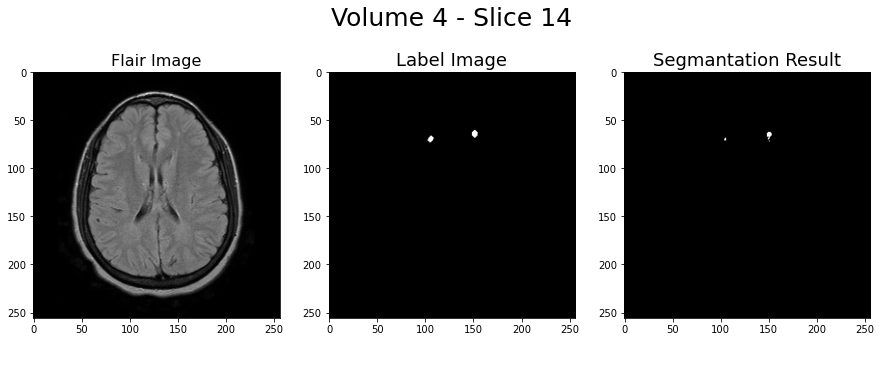
\includegraphics[width = \textwidth]{volume-004-014.png}
\caption{Segmentation result for slice 14 of patient 4.}
\label{fig:volume-004-014}
\end{figure}

\begin{figure}[h!]
\centering
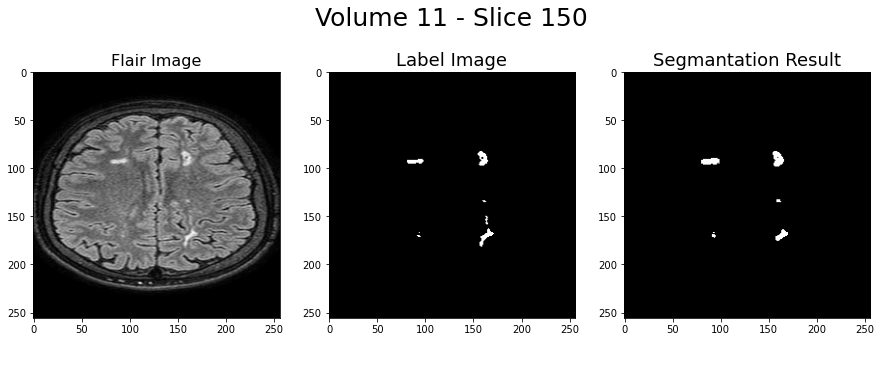
\includegraphics[width = \textwidth]{volume-011-150.png}
\caption{Segmentation result for slice 150 of patient 11.}
\label{fig:volume-011-150}
\end{figure}

\begin{figure}[h!]
\centering
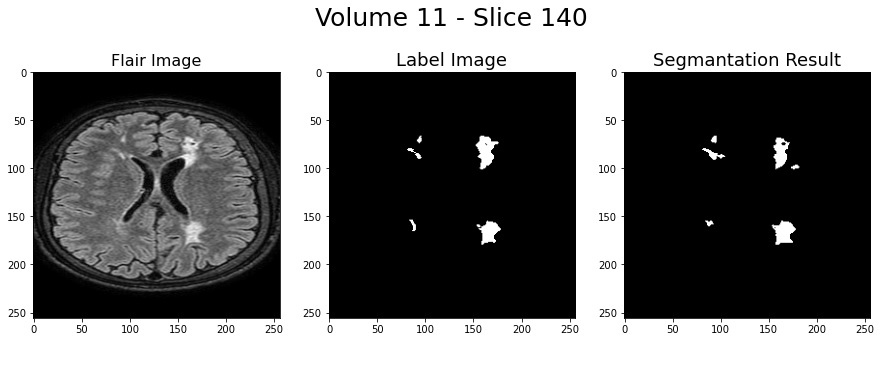
\includegraphics[width = \textwidth]{volume-011-140.png}
\caption{Segmentation result for slice 140 of patient 11.}
\label{fig:volume-011-140}
\end{figure}

\begin{figure}[h!]
\centering
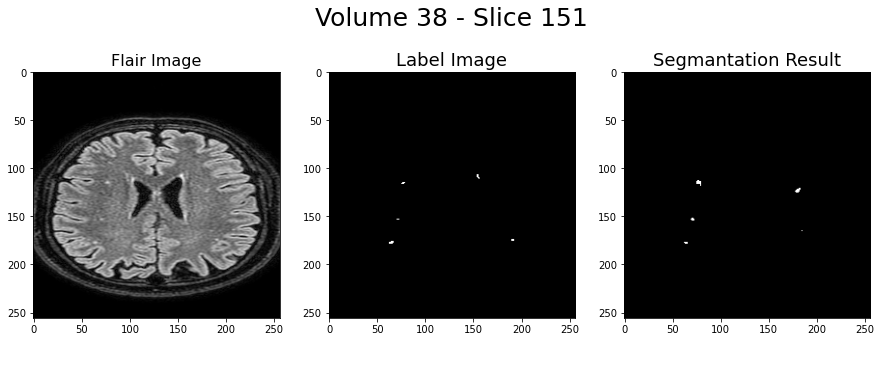
\includegraphics[width = \textwidth]{volume-038-151.png}
\caption{Segmentation result for slice 151 of patient 38.}
\label{fig:volume-038-151}
\end{figure}

\begin{figure}[h!]
\centering
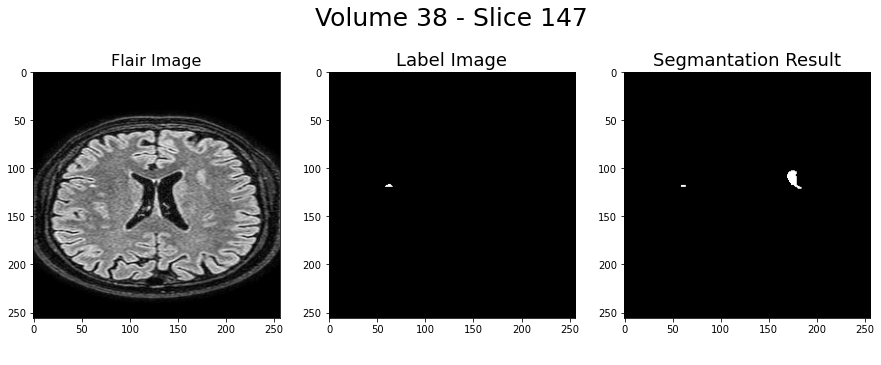
\includegraphics[width = \textwidth]{volume-038-147.png}
\caption{Segmentation result for slice 147 of patient 38.}
\label{fig:volume-038-147}
\end{figure}

\section{Conclusions}
The aim of this work was to implement a neural network algorithm able to detect and segment white matter lesions, that are typically referred to as white matter hyperintensities (WMH), using the hardware offered by CINECA.\\
The algorithm that has been implemented is based on an ensemble model made of three U-Net networks, an example of which is shown in Figure \ref{fig:unet}. As explained in Section \ref{sec:loss_and_param}, three loss functions have been used that are the Dice Loss function in the first model, the Focal Tversky Loss in the second model with $\alpha = 0.7$, $\beta = 0.3$ and $\gamma = 4.0$, and the Binary Focal Loss with a focusing parameter $\gamma$ equal to $2.0$ in the third model. In the first model the learning rate was set to $1\cdot 10^{-5}$ while in the second and third model $1\cdot 10^{-6}$.\\[4pt]
As introduced in Section \ref{sec:data_aug}, random transformations of the training images were used in order to sensibly increase the size of the training dataset, giving to the model robustness to subject rotation and to shear transformations. \\
Giving the fact that the slices containing WMH in the training sample were just a small fraction of the total slices, data augmentation was applied only to slices with lesions, increasing sensibly their number within the training dataset.\\[4pt]
The segmentation results were evaluated by using the Dice Similarity Coefficient, introduced in Section \ref{sec:evaluation_metric}. The distributions of the DSC for the different test patients are shown in Figure \ref{fig:DSC_afterTraining}. 
As already mentioned in Section \ref{sec:results}, some very good results have been obtained referring to slices in which the model correctly detected and segmented the WMHs. 
Aside the good results, in some slices the network showed a poor performance, giving as a result a DSC smaller that $0.2$ and, in some cases, also of the order of $10^{-2}$. \\
This problem could be solved by increasing even more the use of data augmentation in order to let the network be less subjected to variability of different patients and machines used to acquire the images. 
In addition, some images are slightly affected by acquisition artefacts, affecting the performance of the network. \\[4pt]
Unfortunately, it was not possible to increase more the size of the training dataset by using data augmentation due to the fact that CINECA offers a total working time of four hours. After four hours the training session is stopped.
One thing that could be done is to improve the efficiency of the Python code thus managing to greatly reduce the time needed for the network to be trained and make correct predictions.
If the training time is reduced, it will be possible to increase the size of the training dataset by a heavier use of data augmentation.

\clearpage
\bibliographystyle{unsrt}
\bibliography{sample.tex}
\end{document}